\section{Research objective and framework foundations}
Educational responses require separate checks of program facts and task completion. Giving the right output does not diagnose a learner's misconception; a plausible explanation can still give an incorrect follow-up answer. This chapter asks whether synthesized references are executable and traceable, whether filtering reduces superficial preference cues, and which limitations remain. It delivers 1,000 supervised fine-tuning (SFT) demonstrations and 500 preference pairs. Student learning is not measured.

\subsection{NaturalThoughts: which reasoning examples to retain}
NaturalThoughts generates, annotates, selects, and distils reasoning demonstrations~\cite{nat}. Questions sampled from NaturalReasoning receive DeepSeek-R1 reasoning traces and final answers. Domain labels, reasoning strategies such as verification and backtracking, and verbosity distinguish diversity from repeated narration. Selection examines topic/semantic/strategy diversity and difficulty proxies, including disagreement between models with different reasoning behavior. Disagreement does not prove either answer correct. In mixed distillation, disagreement examples retain complete reasoning and other examples can retain only final answers; the selected records supervise a student model.

Its evidence is scale-dependent. With Llama-3.1-8B-Instruct and 100,000 examples, disagreement selection versus random sampling gives 45.2\% versus 42.5\% on GPQA-Diamond; at 500,000 examples, the values are 45.2\% versus 48.3\%~\cite{nat} (p.~7, Table~1). This project borrows separate selection attributes and independent output checks. It does not reproduce DeepSeek-R1 generation, the paper's annotations, or large-model distillation. Structural difficulty labels have no student calibration.

\subsection{Matrix: how heterogeneous generation stages execute}
Matrix wraps each input in a serializable orchestrator containing workflow state, intermediate history, and routing decisions~\cite{matrix}. Queue-driven agent actors update that item and pass it to the next stage; completed items reach a persistent sink. Inference and containerized tools are separate services. Row-level scheduling and data/task/agent parallelism allow individual items to advance without waiting for a heterogeneous batch. Monitoring tracks queues, outstanding work, and latency. Its at-most-once behavior requires recording failures: restarting an actor does not automatically recover a dequeued in-flight item.

In webpage-to-reasoning synthesis, document filtering, question/reference extraction, independent solving, and optional verification are distinct stages. Scheduling does not determine answer quality; task-specific checks do. The paper reports approximately 6.8 times Coral's throughput using the same model and 248 A100 GPUs, with each system's own concurrency and similar reported consensus correctness~\cite{matrix} (p.~9, Table~1). The local implementation borrows separation of stages and per-item provenance; it deploys no distributed Matrix cluster and claims no corresponding speedup.

AIR separates preference annotation, instruction selection, and pairing~\cite{air}; fDPO filters against a current-model-dependent reward comparison~\cite{fdpo}; DEITA combines complexity, quality, and embedding diversity~\cite{deita}. These inform design choices, without importing their thresholds or claiming their model improvements. The cited papers supply the original mechanisms and their evidence boundaries.

\begin{figure}[H]\centering
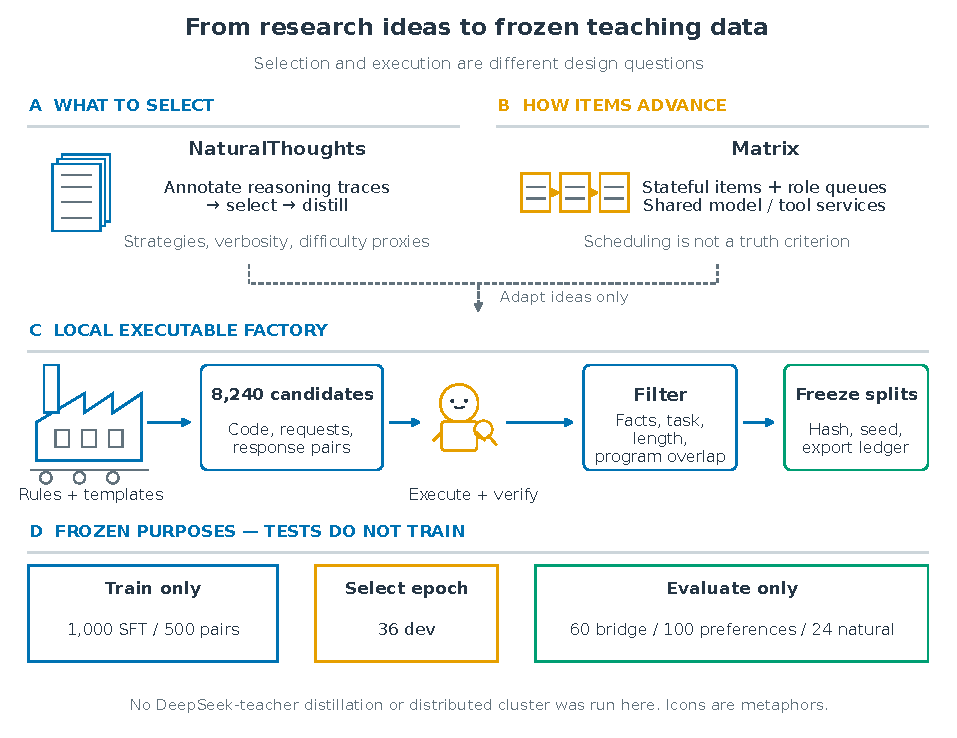
\includegraphics[width=\linewidth]{../../assets/en/synthesis-atlas.pdf}
\caption{From two research inspirations to a bounded executable dataset. The framework contributions, implemented verification, and frozen training/evaluation exports are distinct. The factory and inspector are explanatory metaphors, not additional agents or experimental subjects.}\label{fig:data-pipeline}
\end{figure}\FloatBarrier

\section{Executable data construction and verification}
An SFT record has user/assistant messages; a preference record has a shared prompt and chosen/rejected responses. Metadata binds family, task, structural difficulty, seed, candidate ID, program, reference, filtering decision, and export row. The revised generator records 8,240 candidates across 24 training families. Prediction, explanation, diagnosis, and transfer each receive 250 SFT examples. Negatives comprise 250 factual errors and 250 instruction mismatches, such as omitting an explicitly requested explanation. These rule-constructed contrasts are not naturally sampled model errors. Chinese requests and responses remain unchanged in the frozen files; English examples are translations. No online teacher model generates each row, and there are no student observations or teacher preference votes.

For original program $P$ and follow-up $P'$, independently computed outputs $y,y'$ must satisfy
\begin{equation}
V(P,P')=\mathbf1\{\operatorname{stdout}(P)=y\}\mathbf1\{\operatorname{stdout}(P')=y'\}.
\label{eq:data-exec}
\end{equation}
The auditor uses the standard library without importing the generator/renderer, checks tagged references and negative types, and requires answer-changing variants where intended. Exact normalized programs and prompts are checked across splits, including original/follow-up combinations. A coarser AST measure removes names and constants to expose template repetition; it serves a different purpose from exact deduplication. Shared project authorship still limits independence.

Exports contain 1,000 SFT demonstrations, 500 preference pairs, 36 development demonstrations from three held-out families, 60 byte-preserved earlier bridge references, 100 held-out preference pairs, and 24 separately authored natural questions. Development records select checkpoints; tests do not. Natural questions are Codex-authored within the project and some topics overlap training, so they test new instances/phrasing rather than wholly unseen knowledge. The revised audit passes 11,234 heterogeneous checks and regenerates ten principal files identically. This supports traceability and executable consistency, not an 11,234-item pedagogical pass rate.

\section{Filtering comparison and residual shortcuts}
The earlier release permits a controlled selection study on the same 1,931 eligible preference candidates. Fifty paired permutations compare random selection (A), task/background/defect balancing (B), and additional length priority (C), with fixed family quotas and 500 selected pairs each. Unshuffled C reproduces the published IDs. These are order permutations of one pool, not 50 independently collected datasets. Define
\begin{equation}
H=(n_{\mathrm{preferred\ longer}}+0.5n_{\mathrm{equal}})/N.
\label{eq:data-heuristic}
\end{equation}
The label imbalance $D$ is the family-quota-weighted mean total-variation distance $\frac12\sum_k|p_k-1/K|$ across task, background, and defect axes.

\begin{table}[H]\centering\small
\caption{Selection on one fixed pool: means (sample SD over 50 permutations); $D$ reports means only.}\label{tab:data-ablation}
\begin{tabularx}{\linewidth}{@{}Yrrr@{}}\toprule
Policy & \shortstack{Chosen shorter\\(\%)} & \shortstack{Choose-longer $H$\\(\%)} & $D$\\\midrule
A: random & 19.08 (1.43) & 80.63 (1.44) & 0.1112\\
B: labels & 19.39 (1.03) & 80.31 (1.02) & 0.0189\\
C: length + labels & 43.89 (0.12) & 55.97 (0.15) & 0.0278\\\bottomrule
\end{tabularx}
\end{table}\FloatBarrier

\begin{figure}[H]\centering
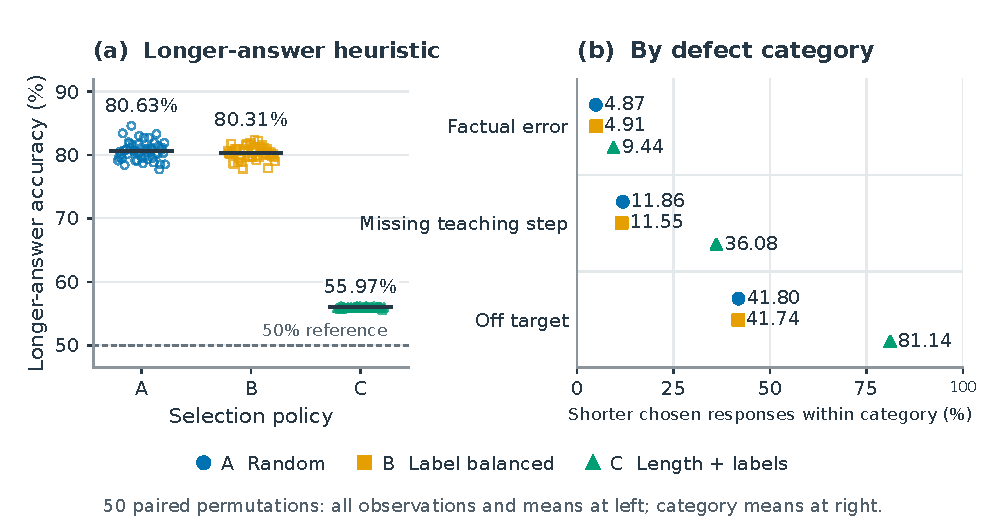
\includegraphics[width=\linewidth]{../../assets/en/selection-ablation.pdf}
\caption{Observed length cues under three selection policies. Points retain all 50 paired permutations; category means expose cues concealed by the aggregate. No model is trained for this comparison.}\label{fig:data-ablation}
\end{figure}\FloatBarrier

Adding length priority reduces $H$ relative to B in every permutation: mean $-24.34$ percentage points, SD 1.02, range $[-26.3,-21.7]$. Label imbalance increases from 0.0189 to 0.0278, documenting a trade-off. Under C, shorter-chosen proportions still differ by negative category: 9.44\% factual errors, 36.08\% teaching omissions, and 81.14\% objective shifts.

Family supply explains why nearest-half balancing does not achieve 250 shorter-chosen pairs. Floor-half targets sum to 245, while list aliasing, loop control, and recursion lack 14, 7, and 5 pairs. Seven odd-quota families can each contribute one extra. Thus the family-nearest-half feasible total is 219--226; the published set has 220 and the permutations 219--221. Overall 250 is possible only by letting some families compensate for others and depart from internal half balance.

\begin{figure}[H]\centering
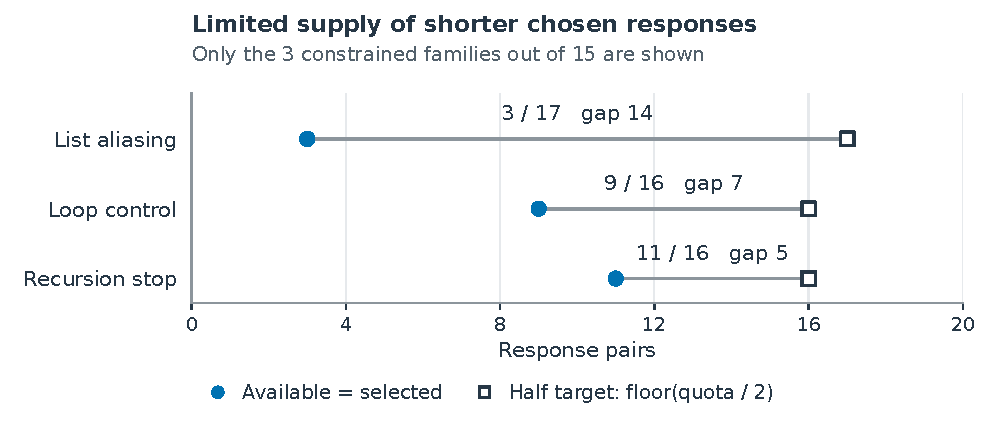
\includegraphics[width=\linewidth]{../../assets/en/family-supply.pdf}
\caption{Three of 15 original training families lack enough shorter-chosen candidates to reach floor-half quotas. All available shorter-chosen pairs in these families are selected; annotated deficits explain the remaining constraint.}\label{fig:data-family-supply}
\end{figure}\FloatBarrier

The original off-topic negatives also leak labels through three mutually exclusive literal fragments: 58 contain \verb|sep='-'|, 62 contain \verb|end=''|, and 59 contain \verb|print('A#B')|. None of the other 321 negatives or 500 chosen responses matches. The revision removes these known cues and shortens responses, but does not prove removal of all shortcuts.

\begin{table}[H]\centering\small
\caption{Published-release diagnostics under matched definitions. The 55.9\% published-set value differs from the 55.97\% permutation mean.}\label{tab:data-revision}
\begin{tabularx}{\linewidth}{@{}Yrr@{}}\toprule
Diagnostic & Earlier & Revised\\\midrule
SFT / preference AST structures & 105 / 98 & 145 / 121\\
Median SFT / chosen characters & 306 / 296 & 65 / 64\\
Choose-longer success & 55.9\% & 50.0\%\\
Negatives with checked fixed cues & 179 & 0\\\bottomrule
\end{tabularx}
\end{table}\FloatBarrier

Residual coupling remains strong: of 250 factual-error negatives, 122 are transfer and 121 diagnosis, versus six prediction and one explanation; all 250 instruction-mismatch negatives are prediction/explanation. The preference test has a related association. All 1,000 SFT answers use the same output label once, reduce to 145 structures, and contain 890 distinct complete responses; the 36 development rows contain only four structures. Executability therefore coexists with limited pedagogical and protocol coverage.

\section{Conclusion and supplementary evidence}
The data study implements generation and filtering and measures specific surface-cue changes. It does not establish improved reasoning, teacher-rated quality, or student learning. Twelve historical qualitative checks are non-blind Codex inspection, not a corpus-wide success estimate. Candidate ledgers, per-item reviews, legacy fingerprint definitions, and the complete C00670 preference example remain in the published synthesis data and comparison records. The downstream model tests the stronger reliability claim in Chapter~\ref{ch:training}.
